
\section{Questions/critique by Max (with input from others)}

\begin{enumerate}
    \item Uncertainty at Low event counts --- is it due statistics? Yes (add uncertainty on uncertainty, mean values, shades) --- it does not matter what those error bars are, because the mean is in the >50 degrees --- meaning there is not directional information to extract if you have 10s of events.
    \item Why is the 5-mm uncertainty consistently larger than 150-mm-segment uncertainty? Answer: Fig 3, neutron travel distance results in sparse matrices for small segment size.
    \item Different convergence for different N and different segment sizes.
    \item V-plots for different iterations.
    \item Add minor grid marks (on log-log plot).
    \item Expand N to 10k and potentially to 100k.
    \item Re-binning from small to large segments might work.
    \item What is the segment size when our results become belieavable...
    \item Sweet spot --- what is the segment size that works best (lowest uncertainty) for directionality.
    \item This method only works if you have a good model of your detector, meaning that you need to have simulated datasets to compare with the true data set. On top of that, you/we can run as many iterations (Monte Carlo) as we want, but we always have a fixed number of events experimentally collected (reference data set).
    \item Chooz --- 
    \item In 2007, 2-reactor scenario --- how reconstructions.
    \item How to do this for multi-core scenario. SMRs. --- this is outside of this paper; however, we can say that we have a preliminary recipe (further study).
    \item Large uncertainty does not mean that the method is bad --- the new method works, whether the old method does not, for low N. We cannot detect at low N. Think of GPS (Gabe's analogy) --- think of position in the store vs on a mountain range.
   \item what is low N, medium N, high N --- can WE quantify? It depends on the segment size. Potentially a topic for a different paper.
   \item At what event count, when can we start answering a question --- which hemisphere the reactor is located? Meaningful directionality.
\end{enumerate}

\subsection{Discussion of potential applications}
Discuss new challenges posed by SMRs (find good recent reference).
Without cooperative monitoring, it is difficult to assess country's plutonium production capability~\cite{Park:2024ykj}.
While long-range nuclear explosion monitoring via neutrinos is not feasible, neutrinos could be a valuable nuclear weapons diagnostics tool and test cite transparency tool --- could directionality add anything?




\section{TO-DO}

\href{https://colab.research.google.com/drive/1VZJIC3z2_7nOzAeaxa6edl2SoWqFfMP8?usp=sharing}{Colab paper\_b\_stats\_package\.ipynb}


Placeholder for plots:
\begin{enumerate}
\item \sout{diagram in picture showing generic 2D segmented detector (vertically oriented, z axis along axial rod direction), XY, and theta defined. Neutrino beam in XY axis, circular arrow indicating rotation of the detector with respect to the beam.}
    \item \sout{Geant4/RAT-PAC 2 screenshot}
    \item \sout{IBD neutron kinetic energy spectrum (from RAT-PAC)} --- Brian
    \item IBD neutron capture 3D XYZ cloud  --- Jackson.
%    \item IBD neutron capture projections, showing the displacement --- or better XY projection of IBD first scatters and countour lines 0.5, 0.8, 0.9, 1.0 fraction of events within those boundaries. Mean and sigma also shown. Angle max, angle mean --- Gabe.
    \item XY plot for IBD neutron capture location (on Li6 only) and countours for fraction of events, e.g. 0.5, 0.9, 1.0 --- Gabe.
    \item Diagram explaining how the old algorithms works (see SANDD 2nd paper Sutanto et al), to make the point that the sum vector is long and is pointing in positive $x$ direction --- Jackson.
    \item \sout{Time and number of scatters prior to reaching thermal energy, time and number of scatters at thermal energy} --- Brian.
    \item \sout{diagram showing original antineutrino direction and emitted IBD neutron (before first scatter) --- make it circular for better readability. antineutrino as a vector inside a circle} --- Gabe.
    \item \sout{to-scale diagram of IBD neutron trajectory (XY projection) with scatters and capture --- Slava. ADD positron track.}
    \item circular 4 plots: without segmentation (perfect reco), .5 segment, 5 cm, 15 cm. indicating directions of the neutron capture with respect to the production point/segment --- Gabe.
    \item table indicating fraction of useful events (e.g. pair that reconstruct in two separate segments) depending on the segment size (ideally want to have an analytic equation) --- Gabe.
    \item to-scale diagram of SANDD grid 7x7 (with IBD vertex at the center cell) --- maybe.
    \item \sout{neutron energy vs time (for a few IBD neutrons)} --- Brian \sout{(to add plots for 0.5\%\ wt ${}^6$Li doped)}
    \item \sout{plot from RAT-PAC: trajectory of neutron}.
    \item \sout{plot from RAT-PAC: timing before capture} --- Brian.
    \item \sout{plot from RAT-PAC: number of neutron bounces before capture.} --- Brian.
    \item 3D plot of capture locations (showing displacement) XYZ --- Jackson.
    \item grid and wheel diagram --- how to represent segmentation on a circle --- Slava.
    \item matrix form --- Slava.
    \item A digram 3$\times$3 with dots representing location of neutron captures, somewhere in the description of the methodology.
    \item Algorithm plots/diagrams
    \item Q-Q plot for statistics test if needed --- Max?
\item Kuiper and/or Watson test plot --- Max.
    \item Prospect original data redrawn (5 cells, and antineutrino direction) --- Slava.
    \item diagram for SANDD 2nd paper~\cite{Sutanto:2021xpo} estimation method (long sum vector) --- Jackson.
    \item final plot on the estimate of antineutrino direction (TBD)
    \item diagram explaining the backgrounds that mimic IBD (focus on a couple most dominant) --- explain how background would likely be isotropic (but some would not) --- everyone, and keep it short.
    \item in the Simulations section, include a plot 3x3 grid or 5x5 grid --- in each cell, a radar plot showing angular distributions for true prompt/capture locations (this is to highlight that a segment adjacent at 0 degree (i.e. the segment (1,0)) to the prompt segment will have a large spread of angles, yet in the segmented detectors they will all be reconstructed as 0-degree angle. Include the angular distribution for the center (prompt) segment as well, which would essentially be like a case for monolithic detector (but maybe not entirely due to short tracks). --- Gabe, Brian.
    \item Another method, see Fig~\ref{fig_array_path} (similar to K-S test, but without using circular statistics); also check file \verb|1969_Cooper_Statistics_...pdf| (Chapter 14, Cooper, Statistics for Experimentalists, Disctribution-Free Tests) --- Jackson.
    \item Jaccard index (Intersection over Union, IoU)  --- Max, Jackson.
\[
\text{Jaccard Index (IoU)} = \frac{|A \cap B|}{|A \cup B|}
\]
    \item
    Structural Similarity Index (SSIM) for 2D matrices --- Max, Jackson.
    \[
\text{SSIM}(x, y) = \frac{(2\mu_x \mu_y + C_1)(2\sigma_{xy} + C_2)}{(\mu_x^2 + \mu_y^2 + C_1)(\sigma_x^2 + \sigma_y^2 + C_2)}
\]
        \item For Bugey 3, Vogel and Beacom report that asymmetry was observed, can we find this thesis: Comparison between simulation and the neutrino data from BUGEY-3 by    Jean-Pierre Cussonneau (Orsay) Apr, 1992. 179 pages. Report  number: LPC-92-T1 --- Slava, Brian, everyone.
        \item Find this paper: MACRO Collaboration, C. Bemporad, in Proceedings of the
Third International Workshop on Neutrino Telescopes, Venice,
1991 \href{https://inspirehep.net/literature/329585}{https://inspirehep.net/literature/329585} --- Slava, everyone.

\item Introduce timing cuts on neutron capture ---  10 $\mu$s for 0.5\%\ and 25 $\mu$s for 0.1\%\ and check how directionality improves (or not) --- Gabe, Brian.
\item \sout{Plot neutron energy vs distance between scatters (Marc thinks it is a good cross-check to ensure we don't have any bug in RAT-PAC2)} --- Brian.
\item Reproduce plot in Bugey 3 thesis for center segment --- Brian
\item V-plot --- [0, $\pi/4$] (zoomed version) --- for different detectors, i.e. segment sizes --- Gabe, Brian.
\item V-plot --- [0, $\pi/4$] --- for each detector varying the number of events --- 10, 100, 1000, $10^4$, $10^5$, $10^6$ (for each curve report uncertainty of the fit) --- Gabe, Brian.
\item Plot uncertainty of the fit (from the V-plot for each detector) vs number of detected IBDs. This will be the final plot to compare with the conventional method (what we had in paper A) --- Gabe, Brian, all.
\item remake the plot from paper A with only focus on the Li6 2D-segmented detectors, compare it with delta phi plot
\item How uncertainty of the fit translates to delta phi (to make an apples-to-apples comparison between two methods)? An idea --- vary the reference angle and report uncertainty of the fit. In other words, how well the minimum of the V-plot is constrained in the phi space --- Jackson, Max, all.

\item Consolidate graphs of CFND for various number of events on one plot (use different markers for  different N) --- Brian.
\end{enumerate}

\section{Procedure}

\begin{enumerate}
    \item Generate IBD pairs  in plastic chunk, i.e. (X, Y) coordinates for the neutron capture --- antineutrino directional is in positive X axis.
    \item Create a 2D square grid (5mmX5mm SANDD, 55mmX55mm ROADSTR, ~15cmX15cm PROSPECT). Finer granularity more useful event for directionality (but affects light transport if segments are long and thin).
    \item Randomize X, Y on a square, this is for the “prompt” vertex (i.e. initial position of the IBD neutron).
    \item Shift the original (X, Y) neutron capture by that displacement.
    \item  Instead of rotating neutrino beam (and regenerating MC data) --- rotate the grid (!). It will tremendously speed up the process.
   \begin{equation}
       x' = \sqrt{x^2 + y^2} \; \cos \theta_\nu
   \end{equation}
   \begin{equation}
       y' = \sqrt{x^2 + y^2} \; \sin \theta_\nu
   \end{equation}
   where $\theta_\nu$ is the direction of incoming antineutrino ``wind'' relative to the detector's $x$ axis. Select $\theta_\nu$ from a set, e.g. $[0^\circ, 1^\circ, 2^\circ, ..., 45^\circ  ]$.
   \item  Now, we will have unique discrete distributions for various neutrino angles relative to the grid - due to the 90-degree rotational symmetry only need to do it in the range of (0, 45) degrees.
   \item do the same for the ``real'' data set select an angle, let's say 21.5$^\circ$.
   \item  Perform the appropriate test: K-S, A-D, or whatever needed, on this data (keeping in mind that it is on a circle, i.e. the 0 angle is the same as 360). The best alignment should be with either the $21^\circ$ or $22^\circ$ data set.
   \item  (optional) I would also add that let us include constraint positron energy in this study. 
Theta of neutrino as a function of (E positron, Theta neutron). Look up Vogel-Beacom formalism. 
Constraining the positron energy (using realistic detector energy resolution) will allow better constraining the incoming antineutrino angle. 
\end{enumerate}

\section{Historic / semiobsolete text}

We first used the Kolmogorov-Smirnoff test at each degree to find the probability that the calibration set for that angle fitted the pretend data from the ``unknown'' direction.
This worked quite well and we did find some improvement in employing the Anderson-Darling test. However, for brevity's sake we decided to pursue the CFND methodology covered in this paper instead. 


% reference-matching example
\begin{figure}[ht]
    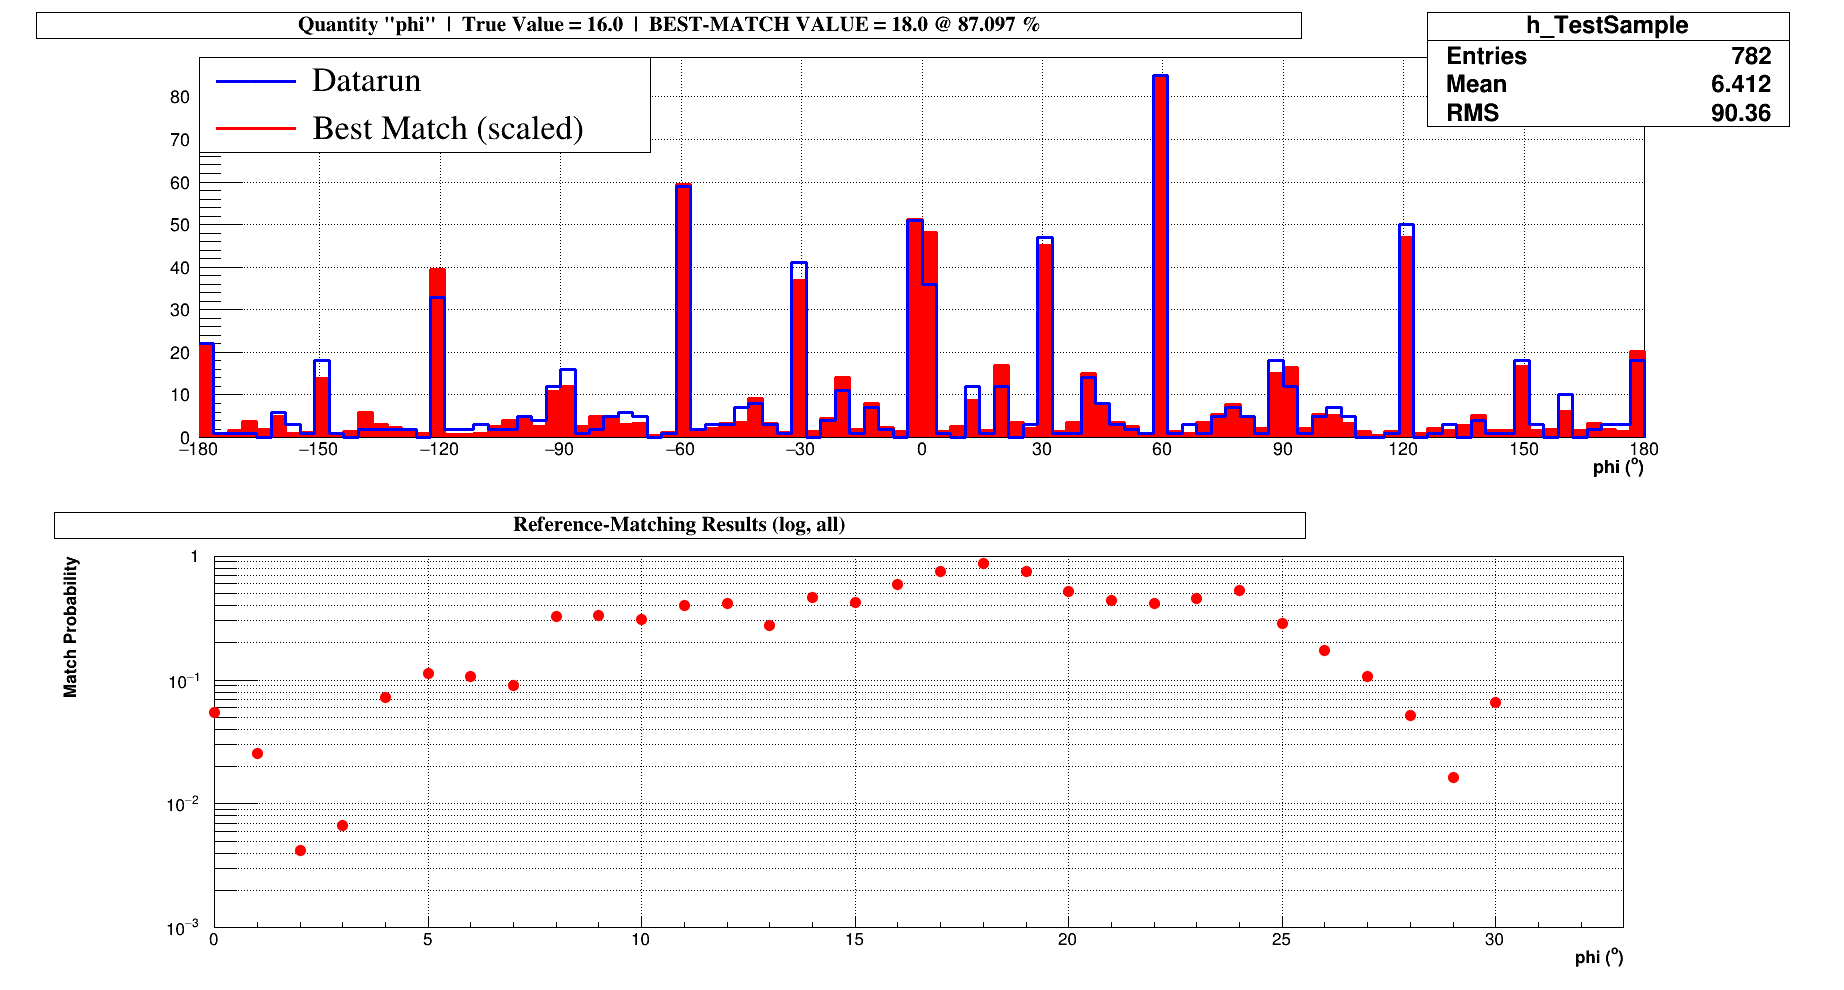
\includegraphics[width=0.8\linewidth]{figures/RefMatchExample_rev2.png}
    \caption{Example of Reference-Matching Algorithm with Antineutrino Source at $16^{o}$}
    \label{fig:ref_example}
\end{figure}

% reference-matching results
\begin{figure}[ht]
    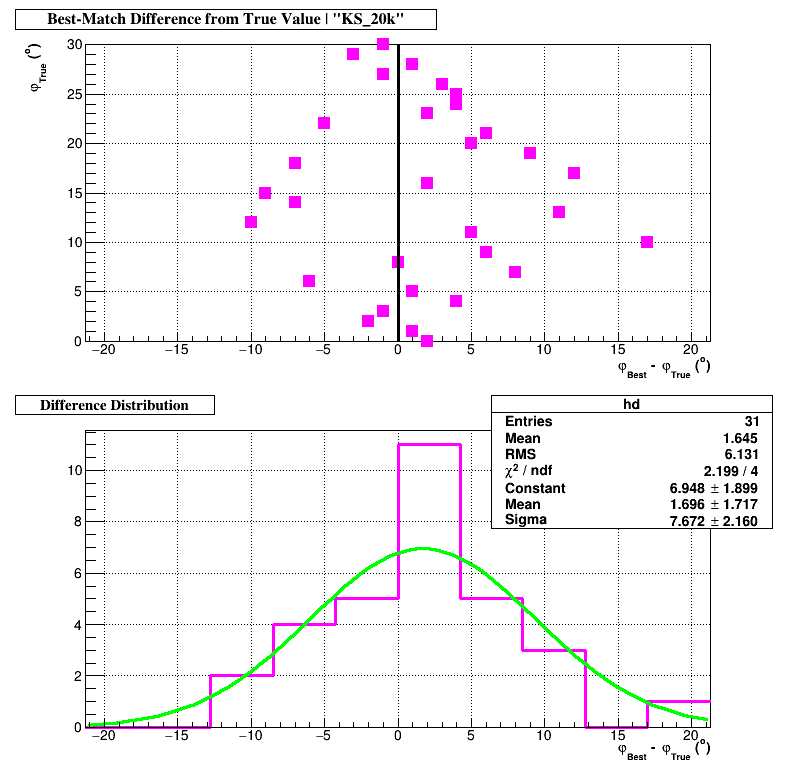
\includegraphics[width=0.8\linewidth]{figures/KS_ref20k.png}
    \caption{Full Results for Matching 1k-Event Test Datasets Against 20k-Event Reference Sets}
    \label{fig:ref_results}
\end{figure}



An example of the results from this reference-matching algorithm is shown in Fig.~\ref{fig:ref_example}.
A summary of the results for the full required set of angles is given in Fig.~\ref{fig:ref_results}.


\section{Experimental --- text/plots in progress...}

Suppose we represent the number of  IBD neutron captures in segments as matrices (the center element is the prompt segment).
\[
A = \begin{pmatrix}
5 & 10 & 15 \\
10 & 0 & 20 \\
5 & 10 & 15
\end{pmatrix}, \ 
B = \begin{pmatrix}
15 & 20 & 15 \\
10 & 0 & 10 \\
5 & 10 & 5
\end{pmatrix}, \ 
C = \begin{pmatrix}
1 & 2 & 3 \\
1 & 0 & 5 \\
1 & 2 & 3
\end{pmatrix}
\]

Normalized:

\[
A_{\text{norm}} = \begin{pmatrix}
0.06 & 0.12 & 0.18 \\
0.12 & 0.00 & 0.24 \\
0.06 & 0.12 & 0.18
\end{pmatrix}
\]

\subsubsection*{Normalized Matrix \( B \)}

\[
B_{\text{norm}} = \begin{pmatrix}
0.18 & 0.24 & 0.18 \\
0.12 & 0.00 & 0.12 \\
0.06 & 0.12 & 0.06
\end{pmatrix}
\]

\subsubsection*{Normalized Matrix \( C \)}

\[
C_{\text{norm}} = \begin{pmatrix}
0.06 & 0.11 & 0.17 \\
0.06 & 0.00 & 0.28 \\
0.06 & 0.11 & 0.17
\end{pmatrix}
\]

Frobenius norm of a matrix $X$ is a square root of the sum of all its elements $x_{ij}$ squared
\begin{equation}
    ||X||_F = \sqrt{\sum \limits_i \sum \limits_j x_{ij}^2}
\end{equation}


Frobenius Norms for the differences:

$A-B$ 	$~\sim$0.24

$A-C$	$~\sim$0.075

$B-C$ 	$~\sim$0.27

Calculate the Differences Between Matrices


1. Difference \( A - B \):
\begin{equation} \nonumber
A - B = \begin{pmatrix}
0.06 - 0.18 & 0.12 - 0.24 & 0.18 - 0.18 \\
0.12 - 0.12 & 0.00 - 0.00 & 0.24 - 0.12 \\
0.06 - 0.06 & 0.12 - 0.12 & 0.18 - 0.06
\end{pmatrix} = 
\end{equation}

\begin{equation}
\begin{pmatrix}
-0.12 & -0.12 & 0.00 \\
0.00 & 0.00 & 0.12 \\
0.00 & 0.00 & 0.12
\end{pmatrix}
\end{equation}

2. Difference \( A - C \):
\begin{equation} \nonumber
A - C = \begin{pmatrix}
0.06 - 0.06 & 0.12 - 0.11 & 0.18 - 0.17 \\
0.12 - 0.06 & 0.00 - 0.00 & 0.24 - 0.28 \\
0.06 - 0.06 & 0.12 - 0.11 & 0.18 - 0.17
\end{pmatrix} = 
\end{equation}

\begin{equation}
\begin{pmatrix}
0.00 & 0.01 & 0.01 \\
0.06 & 0.00 & -0.04 \\
0.00 & 0.01 & 0.01
\end{pmatrix}
\end{equation}


3. Difference \( B - C \):
\begin{equation} \nonumber
B - C = \begin{pmatrix}
0.18 - 0.06 & 0.24 - 0.11 & 0.18 - 0.17 \\
0.12 - 0.06 & 0.00 - 0.00 & 0.12 - 0.28 \\
0.06 - 0.06 & 0.12 - 0.11 & 0.06 - 0.17
\end{pmatrix} = 
\end{equation}

\begin{equation}
\begin{pmatrix}
0.12 & 0.13 & 0.01 \\
0.06 & 0.00 & -0.16 \\
0.00 & 0.01 & -0.11
\end{pmatrix}
\end{equation}


\section*{Step 3: Calculate the Frobenius Norms of the Differences}

1. Frobenius Norm \( \| A - B \|_F \):
\[
\| A - B \|_F = \sqrt{(-0.12)^2 + (-0.12)^2 + (0.12)^2 + (0.12)^2}
\]

\[
= \sqrt{0.0144 + 0.0144 + 0.0144 + 0.0144} = \sqrt{0.0576} \approx 0.24
\]

2. Frobenius Norm \( \| A - C \|_F \):
\[
\| A - C \|_F =  \sqrt{0.0056} \approx 0.075
\]

3. Frobenius Norm \( \| B - C \|_F \):
\[
\| B - C \|_F = \sqrt{0.0728} \approx 0.27
\]

The Frobenius norms for the differences between the matrices are summarized as follows:

\[
\begin{array}{|c|c|}
\hline
\text{Pair of Matrices} & \text{Frobenius Norm} \\
\hline
A - B & \approx 0.24 \\
A - C & \approx 0.075 \\
B - C & \approx 0.27 \\
\hline
\end{array}
\]


Based on the Frobenius norm calculations:
- Matrices \( A \) and \( C \) are the closest to each other with a Frobenius norm of approximately \( 0.075 \).
- Matrices \( A \) and \( B \) are moderately close with a Frobenius norm of approximately \( 0.24 \).
- Matrices \( B \) and \( C \) are the farthest apart with a Frobenius norm of approximately \( 0.27 \).

\subsection{Explanation how grid can be represented on a circle (paper A method}

\subsection{Hypothesis testing}
Our hypothesis is that antineutrino came from a certain angle $\theta_\nu^{exp}$ and caused a distribution of neutron capture in our segments. We want to compare this distribution to a simulated distribution caused by a neutrino at $\theta_\nu^{MC_i}$.


\renewcommand{\arraystretch}{3.5} % Adjusts the height of the rows
\begin{figure}
\noindent 
\begin{minipage}{0.4\linewidth} % Adjust width as needed
\noindent 
%\hspace*{-\leftmargin}
\hspace*{-1.7cm}
\begin{tabular}{|>{\centering\arraybackslash}p{1cm}|>{\centering\arraybackslash}p{1cm}|>{\centering\arraybackslash}p{1cm}|}
    \hline
    $N_{-1}^{1}$ & $N_{0}^{1}$ & $N_{1}^{1}$ \\
    \hline
    $N_{-1}^{0}$ & \sout{$N_{0}^{0}$} & $N_{1}^{0}$ \\
    \hline
    $N_{-1}^{-1}$ & $N_{0}^{-1}$ & $N_{1}^{-1}$  \\
    \hline
\end{tabular}
\end{minipage}%
\begin{minipage}{0.4\linewidth} % Adjust width as needed
%\hspace{.1cm}
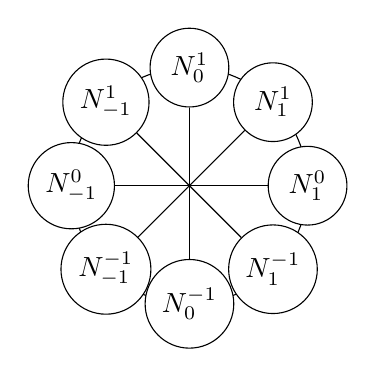
\begin{tikzpicture}
    % Draw the circle
    \draw (0,0) circle (1.5cm);
    % % Define the points on the circle
    % \foreach \i in {0,1,...,7} {
    %     \node at ({360/8 * \i} : 2cm) [circle, draw, fill=white!20] (A\i) {text};
    %     \draw (A\i) -- (0,0); % Draw lines from the circle to the center
    % }
% without for loop
   % Define the points on the circle and draw lines to the center
\node at (0:1.5cm) [circle, draw, fill=white!20, minimum size=1cm] (A0) {$N_{1}^{0}$};
\draw (A0) -- (0,0);

\node at (45:1.5cm) [circle, draw, fill=white!20, minimum size=1cm] (A1) {$N_{1}^{1}$};
\draw (A1) -- (0,0);

\node at (90:1.5cm) [circle, draw, fill=white!20, minimum size=1cm] (A2) {$N_{0}^{1}$};
\draw (A2) -- (0,0);

\node at (135:1.5cm) [circle, draw, fill=white!20, minimum size=1cm] (A3) {$N_{-1}^{1}$};
\draw (A3) -- (0,0);

\node at (180:1.5cm) [circle, draw, fill=white!20, minimum size=1cm] (A4) {$N_{-1}^{0}$};
\draw (A4) -- (0,0);

\node at (225:1.5cm) [circle, draw, fill=white!20, minimum size=1cm] (A5) {$N_{-1}^{-1}$};
\draw (A5) -- (0,0);

\node at (270:1.5cm) [circle, draw, fill=white!20, minimum size=1cm] (A6) {$N_{0}^{-1}$};
\draw (A6) -- (0,0);

\node at (315:1.5cm) [circle, draw, fill=white!20, minimum size=1cm] (A7) {$N_{1}^{-1}$};
\draw (A7) -- (0,0);
\end{tikzpicture}
\end{minipage}
\caption{For clarity a $3\times3$ segment grid is drawn (for small-segment detector grids will be larger, this grid is appropriate for a large-segment detectors such as Prospect). The prompt segment is in the middle, and the number of neutron captures there is $N_{0}^{0}$. If we want to transpose it on circular distribution we won't be using that number, thus it is cross out, i.e.  \sout{$N_{0}^{0}$}.  $N_{x}^{y}$}
\label{fig_segment_table_circle}
\end{figure}

\renewcommand{\arraystretch}{3.5} % Adjusts the height of the rows


\begin{figure}
\begin{picture}(10,10)
        \put(0,0){\color{black}\vector(1,1){20}} 
        \put(10,4){$\bar\nu_e$ ($41^\circ$)}
        \put(0,0){Core (m) (h$\times$d): 0.6 $\times$ 0.4}
\end{picture}
\noindent 
%\hspace*{-\leftmargin}
\hspace*{1.7cm}
\begin{tabular}{|>{\centering\arraybackslash}p{1cm}|>{\centering\arraybackslash}p{1cm}|>{\centering\arraybackslash}p{1cm}|}
    \hline
    --- & 3800 & --- \\
    \hline
    1718 & 39276 & 3766 \\
    \hline
    --- & 2009 & --- \\
    \hline
\end{tabular}

\caption{Prospect data that represent the best directional measurement to date. Prospect does not report/use data for diagonal segments due to low rates. These numbers are from the AAP 2023 presentation, extract proper values from their 2024 paper. }
\label{fig_segment_table_circle}
\end{figure}


\begin{figure}
\begin{picture}(5,5)
        \put(0,0){\color{black}\vector(1,-3){10}} 
        \put(10,4){$\bar\nu_e$ ($\sim -20^\circ$)}
\end{picture}
\noindent 
%\hspace*{-\leftmargin}
\hspace*{1.7cm}
\begin{tabular}{|>{\centering\arraybackslash}p{1cm}|>{\centering\arraybackslash}p{1cm}|>{\centering\arraybackslash}p{1cm}|}
    \hline
    --- & 7.3 \% & --- \\
    \hline
    11.3 \% & 49.8 \% & 11.9 \% \\
    \hline
    --- & 19.7 \% & --- \\
    \hline
\end{tabular}

\caption{Bugey 3 (percentages based on data from inner segments}
\label{fig_Bugey3_percent}
\end{figure}


\begin{table}[]

    \begin{tabular}{|>{\centering\arraybackslash}p{1cm}|>{\centering\arraybackslash}p{1cm}|>{\centering\arraybackslash}p{1cm}|}
    \hline
    --- & 7.3 \% & --- \\
    \hline
    11.3 \% & 49.8 \% & 11.9 \% \\
    \hline
    --- & 19.7 \% & --- \\
    \hline
\end{tabular} \hspace{1cm}
\begin{tabular}{|>{\centering\arraybackslash}p{1cm}|>{\centering\arraybackslash}p{1cm}|>{\centering\arraybackslash}p{1cm}|}
    \hline
    --- & 3800 & --- \\
    \hline
    1718 & 39276 & 3766 \\
    \hline
    --- & 2009 & --- \\
    \hline
\end{tabular}\\\vspace{-0.2cm}

    \begin{tabular}{>{\centering\arraybackslash}p{0.5\linewidth} >{\centering\arraybackslash}p{0.5\linewidth}}
        \makebox[5cm][c]{%
            \begin{picture}(20,20)
                \put(-10,13){\color{black}\vector(1,-3){7}} 
                \put(-40,-20){Bugey: $\theta_\nu \simeq -20^\circ$}
            \end{picture}
        }
        &
        \makebox[5cm][c]{%
            \begin{picture}(20,20)
                \put(-10,-8){\color{black}\vector(1,1){20}} 
                \put(-40,-20){Prospect: $\theta_\nu = 41^\circ$}
            \end{picture}
        }
        \\
    \end{tabular}\\\vspace{0.5cm}

    \caption{Bugey 3 and PROSPECT data. For Bugey, only percentages were originally reported (cite thesis).}
    \label{tab:my_label}
\end{table}

\renewcommand{\arraystretch}{3.5} % Adjusts the height of the rows
\begin{figure}
%\hspace*{-\leftmargin}
%\hspace*{-1.7cm}
\begin{tabular}{|>{\centering\arraybackslash}p{1cm}|>{\centering\arraybackslash}p{1cm}|>{\centering\arraybackslash}p{1cm}|>{\centering\arraybackslash}p{1cm}|>{\centering\arraybackslash}p{1cm}|}
    \hline
    $N_{-2}^{2}$ & $N_{-1}^{2}$ & $N_{0}^{2}$ & $N_{1}^{2}$ & $N_{2}^{2}$ \\
    \hline
    $N_{-2}^{1}$ & $N_{-1}^{1}$ & $N_{0}^{1}$ & $N_{1}^{1}$ & $N_{2}^{1}$ \\
    \hline
    $N_{-2}^{0}$ & $N_{-1}^{0}$ & \sout{$N_{0}^{0}$} & $N_{1}^{0}$ & $N_{2}^{0}$ \\
    \hline
    $N_{-2}^{-1}$ & $N_{-1}^{-1}$ & $N_{0}^{-1}$ & $N_{1}^{-1}$ & $N_{2}^{-1}$ \\
    \hline
    $N_{-2}^{-2}$ & $N_{-1}^{-2}$ & $N_{0}^{-2}$ & $N_{1}^{-2}$ & $N_{2}^{-2}$ \\
    \hline
\end{tabular}
%\hspace{.1cm}
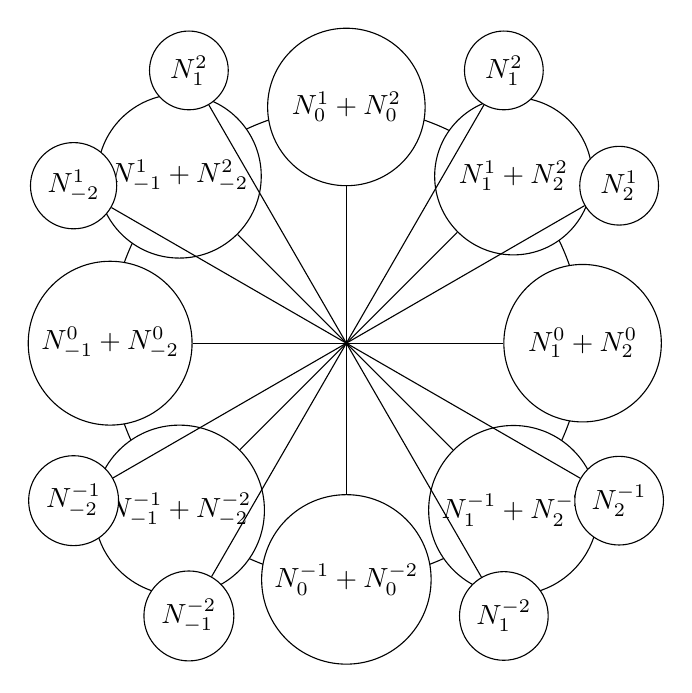
\begin{tikzpicture}
    % Draw the circle
    \draw (0,0) circle (3cm);
    % % Define the points on the circle
    % \foreach \i in {0,1,...,7} {
    %     \node at ({360/8 * \i} : 2cm) [circle, draw, fill=white!20] (A\i) {text};
    %     \draw (A\i) -- (0,0); % Draw lines from the circle to the center
    % }
% without for loop
   % Define the points on the circle and draw lines to the center
\node at (0:3cm) [circle, draw, fill=white!20, minimum size=2cm] (A0) {$N_{1}^{0} + N_{2}^{0}$};
\draw (A0) -- (0,0);

\node at (45:3cm) [circle, draw, fill=white!20, minimum size=2cm] (A1) {$N_{1}^{1} + N_{2}^{2}$};
\draw (A1) -- (0,0);

\node at (90:3cm) [circle, draw, fill=white!20, minimum size=2cm] (A2) {$N_{0}^{1} + N_{0}^{2}$};
\draw (A2) -- (0,0);

\node at (135:3cm) [circle, draw, fill=white!20, minimum size=2cm] (A3) {$N_{-1}^{1} + N_{-2}^{2}$};
\draw (A3) -- (0,0);

\node at (180:3cm) [circle, draw, fill=white!20, minimum size=2cm] (A4) {$N_{-1}^{0} + N_{-2}^{0} $};
\draw (A4) -- (0,0);

\node at (225:3cm) [circle, draw, fill=white!20, minimum size=2cm] (A5) {$N_{-1}^{-1} + N_{-2}^{-2}$};
\draw (A5) -- (0,0);

\node at (270:3cm) [circle, draw, fill=white!20, minimum size=2cm] (A6) {$N_{0}^{-1} + N_{0}^{-2} $};
\draw (A6) -- (0,0);

\node at (315:3cm) [circle, draw, fill=white!20, minimum size=2cm] (A7) {$N_{1}^{-1} + N_{2}^{-2}$};
\draw (A7) -- (0,0);


\node at (30:4cm) [circle, draw, fill=white!20, minimum size=1cm] (A0) {$N_{2}^{1}$};
\draw (A0) -- (0,0);

\node at (60:4cm) [circle, draw, fill=white!20, minimum size=1cm] (A1) {$N_{1}^{2}$};
\draw (A1) -- (0,0);

\node at (120:4cm) [circle, draw, fill=white!20, minimum size=1cm] (A2) {$N_{1}^{2}$};
\draw (A2) -- (0,0);

\node at (150:4cm) [circle, draw, fill=white!20, minimum size=1cm] (A3) {$N_{-2}^{1}$};
\draw (A3) -- (0,0);

\node at (210:4cm) [circle, draw, fill=white!20, minimum size=1cm] (A4) {$N_{-2}^{-1}$};
\draw (A4) -- (0,0);

\node at (240:4cm) [circle, draw, fill=white!20, minimum size=1cm] (A5) {$N_{-1}^{-2}$};
\draw (A5) -- (0,0);

\node at (300:4cm) [circle, draw, fill=white!20, minimum size=1cm] (A6) {$N_{1}^{-2}$};
\draw (A6) -- (0,0);

\node at (330:4cm) [circle, draw, fill=white!20, minimum size=1cm] (A7) {$N_{2}^{-1}$};
\draw (A7) -- (0,0);


\end{tikzpicture}
\caption{A $5\times5$ segment grid. The elements corresponding to the same angle are added, e.g. $N_{1}^{0} + N_{2}^{0}$ (corresponding to 0$^\circ$ angle).}
\label{fig_segment_table_circle}
\end{figure}

\section{Another test to explore}


\begin{figure}[ht]
        \setlength{\unitlength}{.1\linewidth}
%       \setlength{\unitlength}{1cm}
%\fbox{
\begin{picture}(10,10)
%  \thinlines % Start with thin lines
%        \put(0,0){\line(1,0){10}}
        \multiput(1,1)(1,0){10}{\color{gray}\line(0,1){9}} % vertical
        \multiput(1,1)(0,1){10}{\color{gray}\line(1,0){9}} % horizontal
        \multiput(0.5,0.5)(0,1){10}{\color{black}\line(1,0){0.2}} % horizontal ticks
        \multiput(1.5,0.4)(1,0){9}{\color{black}\line(0,1){0.2}} % vertical ticks

        \multiput(0,0)(1,0){9}{\multiput(1.5,1.5)(0,1){9}{\color{black}\circle*{0.1}}} % horizontal
%        \put(4.5,4.50){\color{black}\circle*{0.2}} % 0,0


        \put(.6,0){\vector(0,1){10}} % y axis
        \put(0,.5){\vector(1,0){10}} % x axis

        % \put(5.5,5.5){\color{red}\vector(1,0){1}} % x axis
        % \put(6.5,5.5){\color{red}\vector(0,1){1}} % x axis
        % \put(6.5,6.5){\color{red}\vector(-1,0){1}} % x axis
        % \put(5.5,6.5){\color{red}\vector(-1,0){1}} % x axis
        

% Red unit vectors forming an open loop
        \put(5.5,5.5){\color{red}\vector(1,0){1}} % right

        %first layer
        \put(6.5,5.5){\color{red}\vector(0,1){1}} % up
        \put(6.5,6.5){\color{red}\vector(-1,0){1}} % left
        \put(5.5,6.5){\color{red}\vector(-1,0){1}} % left
        \put(4.5,6.5){\color{red}\vector(0,-1){1}} % down
        \put(4.5,5.5){\color{red}\vector(0,-1){1}} % down
        \put(4.5,4.5){\color{red}\vector(1,0){1}} % right
        \put(5.5,4.5){\color{red}\vector(1,0){1}} % right
   
        %second layes
        \put(6.5,4.5){\color{red}\vector(1,0){1}} % right
        \put(7.5,4.5){\color{red}\vector(0,1){1}} % up


        % \put(6.5,4.5){\color{red}\vector(1,0){1}} % right
        \put(7.5,4.5){\color{red}\vector(0,1){1}} % up
        \put(7.5,5.5){\color{red}\vector(0,1){1}} % up
        \put(7.5,6.5){\color{red}\vector(0,1){1}} % up
  
        \put(6.5,6.5){\color{red}\vector(-1,0){1}} % left

       \multiput(7.5,7.5)(-1,0){4}{\color{red}\vector(-1,0){1}} % left
       \multiput(7.5,3.5)(-1,0){5}{\color{red}\vector(1,0){1}} % right
       \multiput(3.5,7.5)(0,-1){4}{\color{red}\vector(0,-1){1}} % down
  
        % labels
        \put(0,9.8){$y$}
        \put(9.8,0){$x$}

% x labels
        \put(5.4,0){$0$}
        \put(6.4,0){$1$}
        \put(7.4,0){$2$}
        \put(8.4,0){$3$}
        \put(9.4,0){$4$}
        \put(4.1,0){$-1$}
        \put(3.1,0){$-2$}
        \put(2.1,0){$-3$}
        \put(1.1,0){$-4$}

% y labels
        \put(0.2,5.4){$0$}
        \put(0.2,6.4){$1$}
        \put(0.2,7.4){$2$}
        \put(0.2,8.4){$3$}
        \put(0.2,9.4){$4$}
        \put(0,4.4){$-1$}
        \put(0,3.4){$-2$}
        \put(0,2.4){$-3$}
        \put(0,1.4){$-4$}
        
\end{picture}
%} % \fbox
        \caption{Another method to explore --- rectangular spiral. Start with bin (0, 0), assign it index $i = 0$ (follow the red vectors on this diagram), calculate $N_i / N$ (where N is total number of events) in that segment. Potentially, introduce weight $w_i N_i / N$. Calculate max difference between the MC set and empirical set. }
        \label{fig_array_path}
\end{figure}


\section{Kuiper test}

Max comment: issue with coarse binning.
``My hypothesis is that either the python functions are not defined for this 4 cell coarse data, or that we can use n x m buckets for each cell even if they’re degenerate (they map to the same 4 blue cells''

``Since our detector is not a sphere but rectangular—beams normal to a face (0 deg) vs edges (45 deg) I would expect to have different scattering kinematics''



\section{Idea of weight}

Note that the segments for capture that are further away from the prompt provide narrow angles (simple geometry). Therefore, those would ideally constrain better the incoming neutrino direction.
Simple weighting could be done as a square of the distance (in segment units).

Weight will also be impacted by the segment size and the average XY neutron production/capture displacement

\begin{equation}
\begin{pmatrix}
& & 4 & & \\
& \sqrt{2} & 1 & \sqrt{2} & \\
4 & 1 & 0.5 & 1 & 4\\
& \sqrt{2} & 1 & \sqrt{2} & \\
& & 4 & & 
\end{pmatrix}
\end{equation}



% \begin{figure}[ht]
%         \setlength{\unitlength}{.1\linewidth}
% %       \setlength{\unitlength}{1cm}
% %\fbox{
% \begin{picture}(10,5)
% %  \thinlines % Start with thin lines
% %        \put(0,0){\line(1,0){10}}
%         \multiput(5,0)(.5,0){9}{\color{black}\line(0,1){4}} % vertical
%         \multiput(5,0)(0,0.5){9}{\color{black}\line(1,0){4}} % horizontal

%         \multiput(5,4)(.5,0){9}{\color{black}\line(1,1){1}} % horizontal slanted 45-degree
%         \multiput(9,0)(0,.5){9}{\color{black}\line(1,1){1}} % vertical slanted 45-degree

%         \put(10,1){\line(0,1){4}}
%         \put(6,5){\line(1,0){4}}

%         % prompt segment
%           \thicklines
%         \multiput(6.5, 2.50)(.025,0){20}{\color{black}\line(0,1){0.5}} % vertical
%         \multiput(0, 5)(.025,0){20}{\color{black}\line(0,-1){0.5}} % legend
%         % delayed segment
%         \multiput(6, 1.50)(.025,0){20}{\color{gray}\line(0,1){0.5}} % vertical
%         \multiput(0, 4.25)(.025,0){20}{\color{gray}\line(0,-1){0.5}} % legend
%           \thinlines

%         \put(0.8,4.7){prompt segment}
%         \put(0.8,3.9){delayed segment}


%         \put(1,1){\vector(-1,-1){1}} % z axis
%         \put(1,1){\vector(0,1){2}} % y axis
%         \put(1,1){\vector(1,0){2}} % x axis

%         \put(1,1){\vector(2,1){2}} % nu axis
%         \put(1,1){\arc[0,26]{1}} % angle phi_nu
%         \put(1,1){\arc[0,26]{.95}} % angle phi_nu

%         % labels
%         \put(0,0.3){$z$}
%         \put(0.7,2.8){$y$}
%         \put(2.8,.7){$x$}
%         \put(2.7,2){$\nu$}
        
%        \put(6.75,-0.1){\color{black!90}\vector(0,1){4.7}} % y axis
%         \multiput(6.7,0.)(0,.25){16}{\color{blue}\line(1,0){0.1}}
%         \put(4.8,2.75){\color{black!90}\vector(1,0){4.8}} % x axis
%         \multiput(5,2.7)(.25,0){16}{\color{blue}\line(0,1){0.1}} 

%         \put(6.9,4.5){\color{black}$y'$}
%         \put(9.2,2.4){\color{black}$x'$}
%         \put(5.85,2.1){\color{black}$\theta_n^i$}


%         \put(6.75,2.75){\color{blue}\arc[0,245]{0.65}} % angle phi_nu
%         \put(6.75,2.75){\color{blue}\vector(-1,-2){0.5}} % neutron capture

%         %neutrino wind
%         \multiput(3.5, 0.5)(0,1){4}{\color{black}\vector(2,1){1}} % vertical
        
%        \put(2,0){neutrino wind} % nu axis
%         \put(2.2,1.2){$\theta_\nu$}

% \end{picture}
% %} % \fbox
%         \caption{Diagram explaining the prompt-delayed segment geometry, as well as neutrino and axes orientation.
%         In this work we assume that neutrino ``wind'' is in $xy$ plane, at an angle $\nu$ with the $x$ axis.
%         The prompt and delayed segment in this diagram shown for illustrative purposes; the actual separation depends on the segment size --- for large segments, prompt and delayed events would happen in the same segment. It is also illustrated that capture is not necessarily aligned with the neutrino beam (only on average it is the case as discussed in this paper).
%         To study the angular dependence we vary the angle of neutrino with respect to the detector's $x$ and $y$ axes (i.e. rotation of the detector along $z$ axis).}
%         \label{fig:phi_def}
% \end{figure}


% \begin{figure}[ht]
%         \setlength{\unitlength}{.1\linewidth}
% %       \setlength{\unitlength}{1cm}
% %\fbox{
% \begin{picture}(10,5)
% %  \thinlines % Start with thin lines
% %        \put(0,0){\line(1,0){10}}
%         \multiput(5,0)(.5,0){9}{\color{black}\line(0,1){4}} % vertical
%         \multiput(5,0)(0,0.5){9}{\color{black}\line(1,0){4}} % horizontal

%         \multiput(5,4)(.5,0){9}{\color{black}\line(1,1){1}} % horizontal slanted 45-degree
%         \multiput(9,0)(0,.5){9}{\color{black}\line(1,1){1}} % vertical slanted 45-degree

%         \put(10,1){\line(0,1){4}}
%         \put(6,5){\line(1,0){4}}

%         % prompt segment
%           \thicklines
%         \multiput(6.5, 2.50)(.025,0){20}{\color{black}\line(0,1){0.5}} % vertical
%         \multiput(0, 5)(.025,0){20}{\color{black}\line(0,-1){0.5}} % legend
%         % delayed segment
%         \multiput(6, 1.50)(.025,0){20}{\color{gray}\line(0,1){0.5}} % vertical
%         \multiput(0, 4.25)(.025,0){20}{\color{gray}\line(0,-1){0.5}} % legend
%           \thinlines

%         \put(0.8,4.7){prompt segment}
%         \put(0.8,3.9){delayed segment}


%         \put(1,1){\vector(-1,-1){1}} % z axis
%         \put(1,1){\vector(0,1){2}} % y axis
%         \put(1,1){\vector(1,0){2}} % x axis

%         \put(1,1){\vector(2,1){2}} % nu axis
%         \put(1,1){\arc[0,26]{1}} % angle phi_nu
%         \put(1,1){\arc[0,26]{.95}} % angle phi_nu

%         % labels
%         \put(0,0.3){$z$}
%         \put(0.7,2.8){$y$}
%         \put(2.8,.7){$x$}
%         \put(2.7,2){$\nu$}

% % axes for prompt delayed

% \end{picture}
% %} % \fbox
%         \caption{Diagram explaining the prompt-delayed segment geometry, as well as neutrino and axes orientation.
%         In this work we assume that neutrino ``wind'' is in $xy$ plane, at an angle $\nu$ with the $x$ axis.
%         The prompt and delayed segment in this diagram shown for illustrative purposes; the actual separation depends on the segment size --- for large segments, prompt and delayed events would happen in the same segment. It is also illustrated that capture is not necessarily aligned with the neutrino beam (only on average it is the case as discussed in this paper).
%         To study the angular dependence we vary the angle of neutrino with respect to the detector's $x$ and $y$ axes (i.e. rotation of the detector along $z$ axis).}
%         \label{fig:phi_def}
% \end{figure}



\section{Asymptote package for plotting}


\begin{figure}
\centering
\begin{asy}
import graph;
import stats;

size(8.4cm,5cm,IgnoreAspect);
defaultpen(fontsize(10pt));

int n=10000;
real[] a=new real[n];
for(int i=0; i < n; ++i) a[i]=Gaussrand();

// draw(graph(Gaussian,min(a),max(a)),blue);

// Optionally calculate "optimal" number of bins a la Shimazaki and Shinomoto.
int N=bins(a);

histogram(a,0,max(a),N,normalize=false,low=0,white,black,bars=true);

xaxis("Neutron Energy (keV)",BottomTop,LeftTicks);
yaxis("Events",LeftRight,RightTicks(trailingzero));
\end{asy}
    \caption{Spectrum of IBD neutrons. Histogram of kinetic energy of neutrons prior to any scatters as they exit the IBD vertex.}
    \label{}
\end{figure}


\begin{figure}
\centering
\begin{asy}
import graph;
import stats;
size(8.4cm,5cm,IgnoreAspect);
defaultpen(fontsize(10pt));

int n=30;
real[] y=new real[n];
real[] x=new real[n];

real tmp=0.1;
tmp=Gaussrand();
for(int i=0; i < n; i+=2){
x[i]=i;
x[i+1]=i+1;
y[i]=(10*tmp+30)*exp(-i/10);
y[i+1]=(10*tmp+30)*exp(-i/10);
};

draw(graph(x,y),black);
ylimits(0,50);

xaxis("$i$-th segment",BottomTop,LeftTicks);
yaxis("Number of Events $N_i$",LeftRight,RightTicks);
\end{asy}
    \caption{.}
    \label{}
\end{figure}


% \begin{figure}
% \centering
% \begin{asy}
% size(100); // Set the size of the plot
% import graph; // Import the graph module

% // Define the function to plot
% real f(real x) {
%     return x^2; // Example function: y = x^2
% }

% // Draw the axes
% draw((-2,0)--(2,0), Arrow); // x-axis
% draw((0,-1)--(0,4), Arrow); // y-axis

% // Label the axes
% label("$x$", (2,0), E, fontsize(10)); // Label x-axis
% label("$y$", (0,4), N, fontsize(10)); // Label y-axis

% // Plot the function
% draw(graph(f,-2,2), red); // Plot the function in red
% \end{asy}
%     \caption{Caption $x$. This figure is to test font size in plot with asymptote package.}
%     \label{fig:enter-label}
% \end{figure}

% \section{In progress}


% \begin{figure}[ht]
%     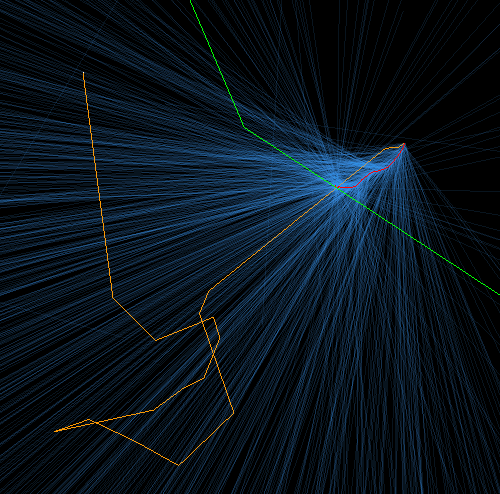
\includegraphics[width=1\linewidth]{fig/RAT_PAC_IBD_run_6_5_crop.png}
%     \caption{Rendering of RAT-PAC 2 IBD visualization. Positron track in red, neutron track --- orange, gamma-rays --- green, Cherenkov photons --- cyan. Scintillation light turned off for clarity. Cherenkov photons indicate the direction of the positron, which was ejected from right top to bottom left in this perspective (neutrino, not shown, is from top right to bottom left.}
%     \label{fig_RATPAC_IBD_visual}
% \end{figure}


% \begin{figure}[ht]
%     \begin{overpic}[width=1.0\linewidth]{fig/RAT_PAC_IBD_run_6_5_crop.png}
    
%     \put(11,90){\color{white}\vector(1,-1){5}}
%     \put(0,93){\fcolorbox{white}{white!30}{\parbox{35pt}{neutron capture}}}
    
%     \put(67,45){\color{white}\vector(0,1){15}}
%     \put(57,41){\fcolorbox{white}{white!30}{\parbox{50pt}{${\color{red}e^+} e^- \to {\color{green}\gamma} \; {\color{green}\gamma}$}}}

%     \put(81,86){\color{white}\vector(0,-1){15}}
%     \put(70,85){\fcolorbox{white}{white!30}{\parbox{60pt}{$\bar\nu_e \; ^1\mathrm{H} \to {\color{red}e^+ } \;{\color{orange}n}$}}}
%     \end{overpic}
%     \caption{Rendering of RAT-PAC 2 IBD visualization. Positron track in red, neutron track --- orange, gamma-rays --- green, Cherenkov photons --- cyan. Scintillation light turned off for clarity. Cherenkov photons indicate the direction of the positron, which was ejected from right top to bottom left in this perspective (neutrino, not shown, is from top right to bottom left.}
%     \label{fig_RATPAC_IBD_visual}
% \end{figure}

\section{Misc: various work in progress}

Other details to add in the intro which might be of relenace:

Recent 2025 DayaBay paper:
"The Daya Bay flux shows good consistency with KI and SM2023 models, but disagrees with HM model. The Daya Bay spectrum, however, disagrees with all model predictions."~\cite{An:2025ufv}
Mention the 5-MeV bump and disagreement with models.
Status of sterile neutrinos.


SNO+ result (including geoneutirnos)
``
The SNO+ collaboration reports its second spectral analysis of reactor antineutrino oscillation using 286 tonne-years of new data.  The measured energies of reactor antineutrino candidates were fitted to obtain the second-most precise determination of the neutrino mass-squared difference $\Delta m^2_{21}$ = $7.96^{+0.48}_{-0.42}$) $\times$ 10$^{-5}$ eV$^2$. 
Constraining $\Delta m^2_{21}$ and $\sin^2\theta_{12}$ with measurements from long-baseline reactor antineutrino and solar neutrino experiments yields $\Delta m^2_{21}$ = ($7.58^{+0.18}_{-0.17}$) $\times$ 10$^{-5}$~eV$^2$ and $\sin^2\theta_{12} = 0.308 \pm 0.013$. %($33.7 \pm 0.8$)$^\circ$. 
This fit also yields a first measurement of the flux of geoneutrinos in the Western Hemisphere, with $73^{+47}_{-43}$ TNU at SNO+. ''

\cite{SNO:2025koj}

\begin{figure}
    \centering
    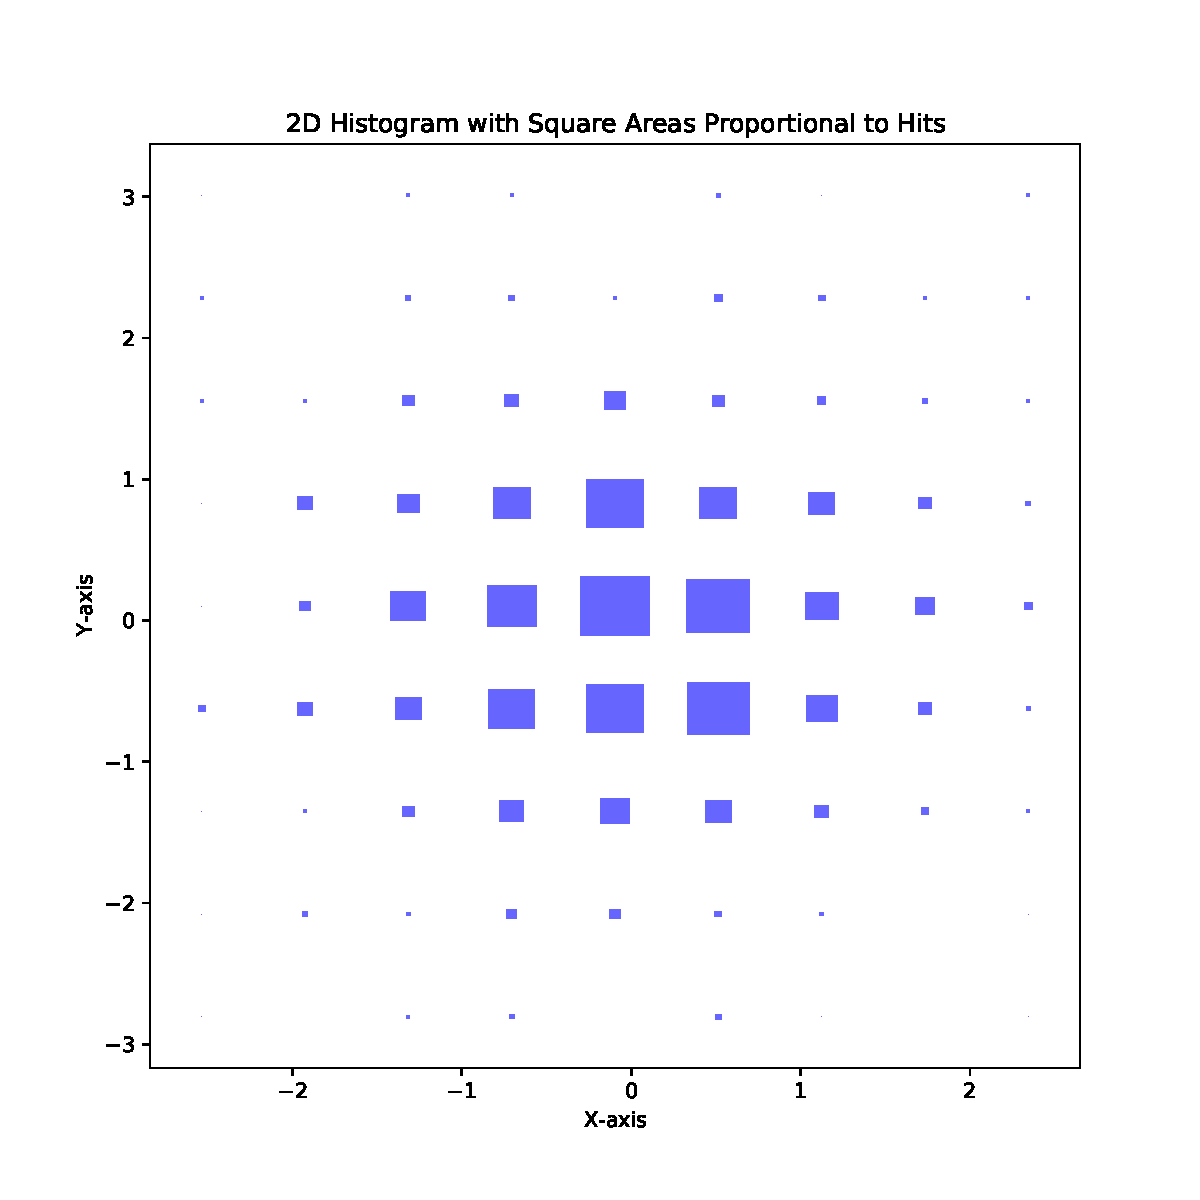
\includegraphics[width=1.0\linewidth]{fig/2d_squares_hist.pdf}
    \caption{Style to represent 2D hist. Area corresponding to number of events. Example of code in LaTeX comments.}
    \label{fig:neutronscattershist}
\end{figure}
% import numpy as np
% import matplotlib.pyplot as plt

% # Generate example data
% x = np.random.normal(size=1000)  # Data for x-axis
% y = np.random.normal(size=1000)  # Data for y-axis

% # Define the number of bins
% x_bins = np.linspace(min(x), max(x), 10)
% y_bins = np.linspace(min(y), max(y), 10)

% # Create a 2D histogram
% hist, x_edges, y_edges = np.histogram2d(x, y, bins=[x_bins, y_bins])

% # Normalize the histogram to scale square sizes
% max_hits = np.max(hist)

% # Plot the histogram
% fig, ax = plt.subplots(figsize=(8, 8))

% for i in range(len(x_edges) - 1):
%     for j in range(len(y_edges) - 1):
%         # Calculate the center of each bin
%         x_center = (x_edges[i] + x_edges[i + 1]) / 2
%         y_center = (y_edges[j] + y_edges[j + 1]) / 2

%         # Scale the square size by the number of hits
%         size = hist[i, j] / max_hits  # Normalize size
%         square_size = size * 0.4  # Adjust scaling factor as needed

%         # Draw the square
%         ax.add_patch(plt.Rectangle((x_center - square_size / 2, y_center - square_size / 2),
%                                     square_size, square_size, color='blue', alpha=0.6))

% # Set axis limits and labels
% ax.set_xlim(x_edges[0], x_edges[-1])
% ax.set_ylim(y_edges[0], y_edges[-1])
% ax.set_xlabel('X-axis')
% ax.set_ylabel('Y-axis')
% ax.set_title('2D Histogram with Square Areas Proportional to Hits')

% plt.savefig("2d_squares_hist.pdf")

